\documentclass[12pt,a4paper,oneside]{article}

\usepackage[utf8]{inputenc}
\usepackage[portuguese]{babel}
\usepackage[T1]{fontenc}
\usepackage{amsmath}
\usepackage{amsfonts}
\usepackage{amssymb}
\usepackage{graphicx}
\usepackage{xcolor}
\usepackage{multicol}
% Definindo novas cores
\definecolor{verde}{rgb}{0.25,0.5,0.35}

\author{\\Universidade Federal de Jataí (UFJ)\\Bacharelado em Ciência da Computação \\Linguagens Formais e Autômatos \\Esdras Lins Bispo Jr.}

\date{07 de novembro de 2019}

\title{\sc \huge Mini-Teste 4}

\begin{document}

\maketitle

{\bf ORIENTAÇÕES PARA A RESOLUÇÃO}

\small
 
\begin{itemize}
	\item A avaliação é individual, sem consulta;
	\item A pontuação máxima desta avaliação é 10,0 (dez) pontos, sendo uma das 06 (seis) componentes que formarão a média final da disciplina: quatro mini-testes (MT), uma prova final (PF) e exercícios aplicados em sala de aula pelo método de Instrução pelos Colegas (IpC);
	\item A média final ($MF$) será calculada assim como se segue
	\begin{eqnarray}
		MF & = & MIN(10, S) \nonumber \\
		S & = & [(\sum_{i=1}^{4} max(MT_i, SMT_i ) + PF].0,2  + IpC\nonumber
	\end{eqnarray}
	em que 
	\begin{itemize}
		\item $S$ é o somatório da pontuação de todas as avaliações, e
		\item $SMT_i$ é a substitutiva do mini-teste $i$.
	\end{itemize}
	\item O conteúdo exigido desta avaliação compreende o seguinte ponto apresentado no Plano de Ensino da disciplina: (3) Autômatos Finitos Não-determinísticos, (6) Gramáticas Livres-de-Contexto e (7) Autômatos com Pilha.
\end{itemize}

\begin{center}
	\fbox{\large Nome: \hspace{10cm}}
\end{center}

\newpage

\begin{enumerate}
	
	\section*{Quarto Teste}
	
	\item {\bf [Sipser 2.14]}  Converta a seguinte GLC numa GLC equivalente na forma normal de Chomsky,
	usando o procedimento apresentado em sala de aula.
	\begin{itemize}
		\item[] $A \rightarrow BAB$ | $B$ | $\epsilon$
		\item[] $B \rightarrow 00$ | $\epsilon$
	\end{itemize}
	
	\item (5,0 pt) Qual das cadeias abaixo este AP \underline{não} aceita? Justifique apropriadamente \underline{todas} as alternativas incorretas.
	
	\begin{center}
		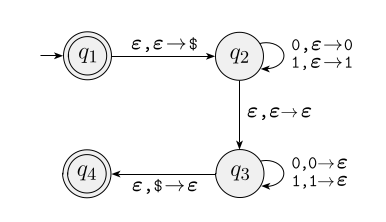
\includegraphics[width=0.5\textwidth]{images/ap3}
	\end{center}
	
	\begin{enumerate}
		\item $\epsilon$
		\item $00$
		\item $11$
		\item $010$ 
		
	\end{enumerate}
	
\end{enumerate}

\end{document}